
\section{Manual técnico}

\subsection*{Obtención de código fuente}

El código fuente de este proyecto se puede obtener por cuatro vías diferentes:

\begin{itemize}
  \item En esta propia documentación, bajo el anexo~\ref{sec:source}.
  \item Del CD que se adjunta al tomo, pegado por la parte interior
	de la portada.
  \item Descargando alguna de las versiones
	publicadas\footnote{\url{http://swaml.berlios.de/files}}.
  \item En el Subversion del proyecto\footnote{\url{http://svn.berlios.de/svnroot/repos/swaml/trunk}} 
	en BerliOS. Puede hacer un \emph{checkout} del repositorio:
	\begin{center}
	 \texttt{svn checkout http://svn.berlios.de/svnroot/repos/swaml/trunk swaml}
	\end{center}
\end{itemize}

\subsection*{Conocimientos}

Antes de abordar el estudio y/o modificación de este proyecto es necesario 
disponga de una serie de conocimientos mínimos acerca de las tecnologías
utilizadas en el mismo.

\begin{itemize}
  \item Debe disponer de conocimientos medios del lenguaje de programación 
	\textbf{Python} en que esta escrito la totalidad del proyecto. 
	Evidentemente se dan por supuestos conocimientos de OOP. En la
	bibliografía podrá encontrar múltiple documentación que le puede ser
	de utilidad.
  \item Conocer bien como funciona el API de 
	\textbf{RDFLib}\footnote{\url{http://rdflib.net/}}, pues el proyecto
	utiliza intensivamente esta biblioteca.
  \item Al menos disponer de nociones básicas sobre 
	\textbf{RDF}\footnote{\url{http://www.w3.org/RDF/}} (Resource Description 
	Framework) y Web Semántica\footnote{\url{http://www.w3.org/2001/sw/}}.
  \item Tener muy presente la especificación de 
	\textbf{SIOC}\footnote{\url{http://rdfs.org/sioc/spec/}} si se necesita
	modifica alguna de las salidas generadas por el proyecto.
\end{itemize}

\subsection*{Continuar con el proyecto}

\begin{figure}[H]
	\centering
	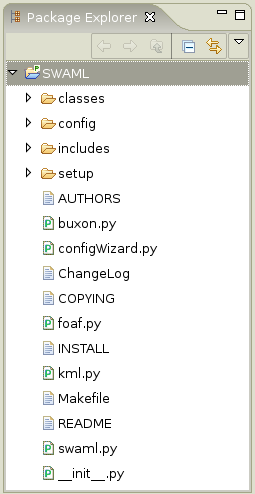
\includegraphics[width=5cm]{images/screenshots/package-explorer.png}
	\caption{Árbol de ficheros del proyecto}
	\label{fig:package-explorer}
\end{figure}

El proyecto se encuentra organizado en dos paquetes: \texttt{swaml} y \texttt{swaml.classes}.
El árbol de ficheros es como el que muestra la figura~\ref{fig:package-explorer}:

\begin{itemize}
  \item En el directorio raíz se encuentran los scripts que sirven como punto de entrada
	a las distintas funcionalidades dadas (paquete\texttt{swaml}).
  \item En el subdirectorio \texttt{classes} se encuentran  todas las bibliotecas de clases
	del proyecto (paquete \texttt{swaml.classes}).
  \item En el subdirectorio \texttt{config} se adjuntan ficheros de configuración de ejemplo.
  \item Bajo el subdirectorio \texttt{includes} están alguno archivos complementarios
	que necesitan las distintas aplicaciones: definición de interfaces gráficas, iconos,
	ficheros de ayuda, etc.
  \item Y en el directorio \texttt{setup} hay una serie de script sólo necesarios en caso
	de que desee instalarse la aplicación.
\end{itemize}

Por tanto, dependiendo de intenciones con que necesita tocarse el código del proyecto,
se deberán modificar ficheros de uno u otro de estos directorios descritos.
